% FORMAT AND PACKAGES
% {
    \documentclass[a4paper]{article}
    \usepackage{a4wide,amssymb,epsfig,latexsym,multicol,array,hhline,fancyhdr}
    \usepackage{vntex}
    \usepackage{amsmath}
    \usepackage{lastpage}
    \usepackage[lined,boxed,commentsnumbered]{algorithm2e}
    \usepackage{enumerate}
    \usepackage{xcolor}
    \usepackage{graphicx}	% Standard graphics package
    \usepackage[table,xcdraw]{xcolor}
    \usepackage{array}
    \usepackage{tabularx, caption}
    \usepackage{multirow}
    \usepackage{multicol}
    \usepackage{rotating}
    \usepackage{graphics}
    \usepackage{geometry}
    \usepackage{setspace}
    \usepackage{epsfig}
    \usepackage[framemethod=tikz]{mdframed}
    \usepackage{tikz}
    \usepackage{xfrac}
    \usepackage{bm}
    \usepackage{biblatex}
    \usepackage[colorlinks]{hyperref}
    \usepackage[utf8]{inputenc}
    % \usepackage[acronym,toc]{glossaries}
    % \usepackage[symbols,nogroupskip,nonumberlist]{glossaries-extra}
    \usepackage[
     sort=none,% no sorting or indexing required
     abbreviations,% create list of abbreviations
     symbols,% create list of symbols
     stylemods,style=list, % set the default glossary style
     nogroupskip, nonumberlist, nomain
    ]{glossaries-extra}
    \usetikzlibrary{patterns}
    \usepackage{pgfplots}
    \pgfplotsset{compat=1.17}
    
    % FORMATTING
    % {
    \DeclareMathOperator{\arccot}{arccot}
    \captionsetup[table]{name=Table}
    \captionsetup[figure]{name=Figure}
    \newenvironment{Description}{\list{}{%
        \let\makelabel\descriptionlabel    % this comes from the original description environment
        \setlength{\rightmargin}{\leftmargin}% this comes from the original quote environment
        \setlength{\labelwidth}{0pt}%          this is new
        }}{\endlist}
    
    \addbibresource{citations.bib}
        
    \hypersetup{urlcolor=blue,linkcolor=black,citecolor=black,colorlinks=true} 
    \usetikzlibrary{arrows,snakes,backgrounds}
    \definecolor{mathblue}{RGB}{0,114,188}
    % \makeatletter  \def\m@th{\mathsurround\z@\color{mathblue}} \makeatother
    % \everymath{\color{mathblue}}
    % \setmathfont[Color=000000]{Arial}
    %\usepackage{pstcol} 								% PSTricks with the standard color package
    \newtheorem{theorem}{{\bf Theorem}}
    \newtheorem{property}{{\bf Property}}
    \newtheorem{proposition}{{\bf Proposition}}
    \newtheorem{corollary}[proposition]{{\bf Corollary}}
    \newtheorem{lemma}[proposition]{{\bf Lemma}}
    
    \AtBeginDocument{\renewcommand{\listfigurename}{List of Figures}}
    \AtBeginDocument{\renewcommand{\listtablename}{List of Tables}}
    \AtBeginDocument{\renewcommand*\contentsname{Contents}}
    \AtBeginDocument{\renewcommand*\refname{References}}
    %\usepackage{fancyhdr}
    
    \setlength{\headheight}{40pt}
    \pagestyle{fancy}
    \fancyhead{} % clear all header fields
    \fancyhead[L]{
     \begin{tabular}{rl}
        \begin{picture}(25,15)(0,0)
        \put(0,-8){\includegraphics[width=8mm, height=8mm]{Image/hcmut.png}}
        %\put(0,-8){\epsfig{width=10mm,figure=hcmut.eps}}
       \end{picture}&
        %\includegraphics[width=8mm, height=8mm]{Image/hcmut.png} & %
        \begin{tabular}{l}
            \textbf{\bf \ttfamily University of Technology, Ho Chi Minh City}\\
            \textbf{\bf \ttfamily Faculty of Computer Science and Engineering}
        \end{tabular} 	
     \end{tabular}
    }
    \fancyhead[R]{
        \begin{tabular}{l}
            \tiny \bf \\
            \tiny \bf 
        \end{tabular}  }
    \fancyfoot{} % clear all footer fields
    \fancyfoot[L]{\scriptsize \ttfamily Assignment for Mathematical Modeling - Academic year 2024 - 2025}
    \fancyfoot[R]{\scriptsize \ttfamily Page {\thepage}/\pageref{LastPage}}
    \renewcommand{\headrulewidth}{0.3pt}
    \renewcommand{\footrulewidth}{0.3pt}
    
    \setcounter{secnumdepth}{4}
    \setcounter{tocdepth}{4}
    
    \makeatletter
    \newcounter {subsubsubsection}[subsubsection]
    \renewcommand\thesubsubsubsection{\thesubsubsection .\@alph\c@subsubsubsection}
    \newcommand\subsubsubsection{\@startsection{subsubsubsection}{4}{\z@}%
                                         {-3.25ex\@plus -1ex \@minus -.2ex}%
                                         {1.5ex \@plus .2ex}%
                                         {\normalfont\normalsize\bfseries}}
    \newcommand*\l@subsubsubsection{\@dottedtocline{3}{10.0em}{4.1em}}
    \newcommand*{\subsubsubsectionmark}[1]{}
    % \def\m@th{\mathsurround\z@\color{mathblue}}
    \makeatother
    % }
    % }
    
    % ACRONYMS & SYMBOLS
    % {
    % \makeglossaries
    \setabbreviationstyle{long-short}
    \newabbreviation{ode}{ODE}{(First-Order) Ordinary Differential Equation}
    \newabbreviation{ivp}{IVP}{Initial-Value Problem}
    \newabbreviation{lte}{LTE}{Local Truncation Error}
    \newabbreviation{ds}{DS}{Dynamical System}
    \newabbreviation{fig}{Fig.}{Figure}
    \newabbreviation{tab}{Tab.}{Table}
    \newabbreviation{sys}{Sys.}{System of Equations}
    \newabbreviation{eq}{Eq.}{Equation}
    \newabbreviation{eg}{e.g.}{For Example}
    \newabbreviation{ie}{i.e.}{That Is}
    \newabbreviation{ILP}{ILP}{Integer Linear Programing problem}
    \newabbreviation{RL}{RL}{Reinforcement learning}
    \newabbreviation{st}{s.t.}{Subject to (in context of ILP)}
    \newabbreviation{PPO}{PPO}{Proximal policy optimization (in context of RL)}
    \newabbreviation{CNN}{CNN}{Convolutional neural network}
    % \glsnoexpandfields
    \glsxtrnewsymbol[description = {Set of natural numbers}]{natural}{\ensuremath{\mathbb{N}}}
    \glsxtrnewsymbol[description = {Set of real numbers}]{real}{\ensuremath{\mathbb{R}}}
    \glsxtrnewsymbol[description = {Set of positive real numbers}]{real_positive}{\ensuremath{\mathbb{R}^+}}
    
    % }
    
    % ^ above is pure header declaration

    % DOCUMENT
    \begin{document}
    
    % TITLE PAGE
    \begin{titlepage}
    \begin{center}
    VIETNAM NATIONAL UNIVERSITY, HO CHI MINH CITY \\
    UNIVERSITY OF TECHNOLOGY \\
    FACULTY OF COMPUTER SCIENCE AND ENGINEERING
    \end{center}
    
    \vspace{1cm}
    
    \begin{figure}[h!]
    \begin{center}
    \includegraphics[width=3cm]{Image/hcmut.png}
    \end{center}
    \end{figure}
    
    \vspace{1cm}
    
    
    \begin{center}
    \begin{tabular}{c}
    \multicolumn{1}{l}{\textbf{{\Large MATHEMATICAL MODELING (CO2011)}}}\\
    ~~\\
    \hline
    \\
    \multicolumn{1}{l}{\textbf{{\Large Assignment}}}\\
    \\
    \textbf{\textit{{\Huge “Cutting stock problem”}}}\\
    \\
    \hline
    \end{tabular}
    \end{center}
    
    \vspace{2cm}
    
    \begin{table}[h]
    \centering
        \begin{tabular}{rl}
        \hspace{3 cm}\textbf{Instructor(s)}:
        & Nguyễn An Khương\\

        & \\[10pt]
        \hspace{3 cm}\textbf{Report team}:
        & Group TN01\_TN - Team 104\\
        \textbf{Students}: 
        &  Bùi Ngọc Minh - 2312046 \emph{(\textbf{Leader})} \\
        &  Lê Trọng Thiện - 2313233\\
        &  Phạm Lê Tiến Đạt - 2310687\\
        &  Lương Minh Thuận - 2313348\\
        &  Nguyễn Đăng Hiên - 2310936\\
        \end{tabular}
    \end{table}
    
    \begin{center}
    {\footnotesize HO CHI MINH CITY, DECEMBER 2024}
    \end{center}
    \end{titlepage}
    
    \pagebreak
    \tableofcontents
    \pagebreak
    
    % Glossaries
    % {}
    \printunsrtglossary[type={symbols}, title={List of Symbols}]
    \printunsrtglossary[type={abbreviations}, title={List of Acronyms}]
    \pagebreak
    \listoffigures
    \listoftables
    \pagebreak
    \addcontentsline{toc}{section}{\listfigurename}
    \addcontentsline{toc}{section}{\listtablename}
    
    % }
    
    % Member list
    \section*{Member list \& Workload}
    \addcontentsline{toc}{section}{Member list \& Workload}
    \begin{center}
    \begin{table}[h]
    \centering
    \begin{tabular}{|c|c|c|p{6cm}|c|}
    \hline
    \textbf{No.} & \textbf{Full name} & \textbf{ID} & \textbf{Problems} & \textbf{\% done}\\
    \hline 
    %%%%%Student 1%%%%%%%%%%
    \multirow{4}{*}{1} & \multirow{4}{*}{Bùi Ngọc Minh} & \multirow{4}{*}{2312046} & 
    - Formulation of the 2D CSP as an ILP,& \multirow{4}{*}{100\%}\\
     & &  &including the restricted 2D knapsack problem&\\
     & &  &- Algorithm research (Theory behind RL and PPO)&\\
     & &  & - \LaTeX  &\\
    \hline 
    %%%%%Student 2%%%%%%%%%%%
    \multirow{4}{*}{2} & \multirow{4}{*}{Lê Trọng Thiện} & \multirow{4}{*}{2313233} & 
    - Algorithm research \& implementation (Combination heuristic derived from best fit and first fit algorithm) & {100\%} \\
    \hline
    %%%%%Student 3%%%%%%%%%%%
    \multirow{4}{*}{3} & \multirow{4}{*}{Phạm Lê Tiến Đạt} & \multirow{4}{*}{2310687} & 
    - Algorithm research \& implementation (Simplex optimization on a predefined set of cutting patterns heuristic) & {100\%}\\
    \hline
    %%%%%Student 4%%%%%%%%%%%
    \multirow{4}{*}{4} & \multirow{4}{*}{Lương Minh Thuận} & \multirow{4}{*}{2313348} & 
    - Algorithm research \& implementation& \multirow{4}{*}{100\%}\\
     & &  & (RL, training via PPO) &\\
     & &  & - Collect benchmark data on the different policies &\\
     & &  & &\\
    \hline
    %%%%%Student 5%%%%%%%%%%
    \multirow{4}{*}{5} & \multirow{4}{*}{Nguyễn Đăng Hiên} & \multirow{4}{*}{2310936} & 
    - Algorithm research (first fit and best fit heuristics)  & \multirow{4}{*}{100\%}\\
    & &  & - Case study of a real life instance of the 2D CSP (Real life data collection and problem formulation)  &\\
    & &  & - \LaTeX  &\\
    \hline
    \end{tabular}
    \caption{\label{table1}Member list \& workload}
    \end{table}
    \end{center}
    
    
    \pagebreak
    
    
    \section{Introduction and Motivation}

    \subsection{The Cutting-Stock Problem}

    The Cutting-Stock Problem is a well-known NP-hard optimization problem with significant real-world implications. It can be stated as follows:
    \vspace{0.2cm}\\
    Given a set of stock materials with fixed dimensions and a list of items to be cut from these stocks with specified dimensions and demands, 
    determine a cutting pattern that minimizes the total number of stocks used or the amount of waste generated. The goal is to meet all demands while optimizing resource utilization.
    \vspace{0.2cm}\\
    This problem frequently arises in industries such as manufacturing, logistics, and supply chain management, where raw materials such as sheets, rods, or rolls need to be cut into smaller pieces efficiently. 
    \vspace{0.2cm}\\
    The Cutting-Stock Problem is typically formulated as an Integer Linear Programming (ILP) problem. Various techniques have been proposed to solve it, including branch-and-bound algorithms, heuristic methods, and column generation approaches with trade off between computational complexity and solution quality between them.
    \vspace{0.2cm}\\
    For simplicity, this big assignment only focuses on a specific variation of the problem, namely the a variation of the 2D Cutting-Stock Problem with each items being non-rotatable 2D rectangles whose dimensions are all integers.

    \subsection{Reinforcement Learning}

    Reinforcement Learning (RL) is a subfield of machine learning that focuses on training an agent to interact with a dynamic environment. The agent learns to take actions that maximize its cumulative reward through trial-and-error interactions. Unlike supervised learning, RL does not require explicit labeling of data or immediate corrections for incorrect behavior. Instead, it relies on feedback in the form of rewards or penalties to guide the agent toward optimal behavior.
    \vspace{0.2cm}\\
    One advantage of RL is its ability to adapt to complex, high-dimensional problems where traditional methods struggle. In the context of the Cutting-Stock Problem, RL offers the potential to dynamically generate cutting patterns by learning from past performance, 
    which could lead to new innovative and efficient solutions.

    \subsection{Motivation}

    Our group’s objectives in this project are to:

    \begin{itemize}
        \item \textbf{1)} Formalize the Cutting-Stock Problem as an ILP, providing a clear mathematical representation of the problem constraints and objectives.
        \item \textbf{2)} Analyze, discuss, and implement different approaches to solving the problem, including traditional optimization techniques and a Reinforcement Learning-based approach. 
        These perspective allows us to compare the strengths and weaknesses of both methods in tackling this challenging problem.
        \item \textbf{3)} Propose potential extensions to our model and exploring its applications in real life situations and demands.
    \end{itemize}

    \noindent By combining insights from different approaches, this project aims to develop a comprehensive understanding of the Cutting-Stock Problem and its potential solutions. 
    We hope that our work will contribute to the broader field of Operations Research and inspire future applications of machine learning in industrial problems.

    \pagebreak
    \section{Acknowledge}

    Our group expresses deep gratitude to our instructor, Mr. Nguyễn An Khương for his guidance and valuable feedback throughout the creation process of this big assignment. 
    \vspace{0.2cm}\\
    We would also like to thank the whole of HCMUT community of students and lecturers, whose questions and answers on the forum helped push the project through hard decisions and ambiguity.

    \pagebreak
    \section{Algorithm}
    \subsection{Heuristic Algorithms}
    Heuristic algorithms are problem-solving methods that focus on finding approximate solutions efficiently, especially in scenarios where exact solutions are computationally expensive or infeasible. These methods rely on rules of thumb, domain knowledge, or practical strategies to reduce the complexity of the search space. By strategically ignoring less promising solutions, heuristics aim to provide good, though not necessarily optimal, results within a reasonable time frame.
    \vspace{0.2cm}\\
    In the context of the Cutting-Stock Problem, heuristic algorithms are instrumental in generating feasible cutting patterns while balancing computational effort and solution quality. This is achieved by incorporating constraints, such as limiting the number of cutting stages or enforcing specific cutting styles like guillotine cuts. These constraints significantly simplify the problem by reducing the vast space of potential cutting patterns, allowing for practical solutions that meet demand and minimize material waste. Despite their approximate nature, heuristics are often highly effective in real-world industrial applications, where quick decisions and resource optimization are paramount.
    \vspace{0.2cm}\\
    Heuristic methods are widely applied in solving two-dimensional cutting and packing problems due to their ability to provide high-quality solutions within a reasonable computational time. These methods are particularly relevant to the Cutting-Stock Problem, as they offer efficient ways to handle its NP-hard nature without requiring an exhaustive exploration of the solution space.

    \subsubsection{Constructive Heuristics}
    Constructive heuristics build solutions incrementally by placing items into stock one at a time. Three classical strategies that have laid the foundation for many solution methods are:  
    \begin{itemize}
        \item \textbf{First-Fit Algorithm:} This method places each item in the first available space or bin that can accommodate it without violating constraints. It is simple, computationally efficient, and often used as a baseline for comparison in packing problems. While not guaranteed to produce optimal solutions, it provides a quick and feasible layout that can be further refined using advanced techniques.  
        \item \textbf{Bottom-Left Algorithm:} This method places items sequentially in the lowest possible position, left-justified. It is effective for structured packing problems, where straightforward placement rules lead to reasonably efficient layouts with minimal computational effort.  
        \item \textbf{Best-Fit Approach:} This method selects items that best fit into the lowest available space during each placement. By focusing on optimal utilization of stock material, it enhances efficiency and reduces waste, making it particularly suitable for resource-constrained problems.  
    \end{itemize}  
    Efficient implementations of these algorithms have been extensively studied. For instance, Chazelle and Imahori \& Yagiura proposed optimized versions to improve computational performance while maintaining solution quality. These constructive heuristics serve as the building blocks for more sophisticated methods and are often used to generate initial solutions in hybrid algorithms.
    \vspace{0.2cm}\\
    As seen in the source code provided in the description of this assignment, the approach of the source code is primarily designed around the First-Fit method, which will be discussed in more detail in the next section of the report.
    
    \subsubsection{First-Fit Algorithm for 2D Cutting-Stock}

    The \textbf{First-Fit Algorithm} is a straightforward heuristic used to solve 2D cutting-stock problems, where the goal is to allocate rectangular items (or products) onto stock sheets in a way that minimizes waste. The algorithm prioritizes placing each product on the first stock sheet that can accommodate it, balancing simplicity and efficiency. Although the solution is not guaranteed to be optimal, it is computationally efficient and feasible for many practical scenarios.
    
    The algorithm operates as follows:
    \begin{enumerate}
        \item \textbf{Product Selection:} Products are placed one by one, in the order they are provided.
        \item \textbf{Find the First Suitable Stock:} For each product, the algorithm checks each available stock sheet (in the order they are considered) to determine if the product can fit, based on the stock's remaining available area and dimensions.
        \item \textbf{Place the Product:} If the product can fit on an existing stock sheet, it is placed there. If no existing stock sheet can accommodate the product, a new stock sheet is introduced, and the product is placed on it.
        \item \textbf{Continue:} The process repeats until all products have been placed.
    \end{enumerate}
    
    Let:
    \begin{itemize}
        \item \( n \) be the number of products to cut.
        \item \( m \) be the number of stock sheets used.
        \item \( W_i, H_i \) be the width and height of the \( i \)-th product.
        \item \( W_j^{\text{stock}}, H_j^{\text{stock}} \) be the width and height of the \( j \)-th stock sheet.
    \end{itemize}
    \vspace{0.2cm}
    The objective of the First-Fit Algorithm for 2D Cutting-Stock is to minimize the number of stock sheets required, while ensuring that the placement respects the dimensions and capacities of the stock sheets. The placement process can be formalized as:
    \begin{enumerate}
        \item Find the first stock sheet \(j\) such that (\(W_i \leq \) remaining width) and (\(H_i \leq\) remaining height).
        \item If no existing stock sheet can accommodate the product, a new stock sheet is created, then \(m = m + 1 \) (introduce a new stock sheet).
    \end{enumerate}    
    \vspace{0.2cm}
    This approach can be enhanced with additional strategies for handling rotation of products, prioritizing smaller items, or rearranging the placement order to achieve better results.
    \vspace{0.2cm}\\
    The main idea is to cut from the largest stock to the smallest stock, and from the largest product to the smallest product, in such a way that the area cut from the stock changes as little as possible. Therefore, the following pseudo code outlines the First-Fit Algorithm. The time complexity of the First-Fit algorithm for 2D Cutting-Stock is \( O(n \cdot m) \), where:
    \begin{itemize}
        \item \( n \) is the number of products to be placed.
        \item \( m \) is the number of stock sheets used.
    \end{itemize}

    \pagebreak
    \begin{mdframed}[backgroundcolor=black!10]
        \begin{tabbing}
    \hspace{0.5cm}\=\hspace{0.5cm}\=\hspace{0.5cm}\=\hspace{0.5cm}\=\hspace{0.5cm}\=\kill
        \textbf{Function} First\_fit\_2DCSP: \\    
        \> \textbf{push} one of each stock\_type into the stock\_list.\\
        \> \textbf{for} $stock_i$ \textbf{from} the largest \textbf{to} smallest area in stock\_list:\\
        \>\> \textbf{for} $prod_j$ \textbf{from} the largest \textbf{to} smallest area in product\_list:\\
        \>\>\> \textbf{if} $prod_j$ \textbf{can fit} into $stock_i$:\\
        \>\>\>\> \textbf{place} $prod_j$ \textbf{into} $stock_i$\\
        \>\>\> \textbf{else}:\\
        \>\>\>\> \textbf{let} ``stockType'' \textbf{be} the first stock\_type that \textbf{fits} $prod_j$\\
        \>\>\>\> \textbf{create} a new stock of type ``stockType''\\
        \>\>\>\> \textbf{place} $prod_j$ \textbf{into} the new stock\\
        \>\>\> \textbf{if} the textbf{demand} for $prod_j$ is textbf{met}:\\
        \>\>\>\> \textbf{remove} $prod_j$ \textbf{from} the item list
        \end{tabbing}
    \end{mdframed}
    
    \vspace{0.2cm}
    Each product might require checking all existing stock sheets to find a place, and if no stock sheet is suitable, a new stock sheet is introduced.
    \vspace{0.2cm}\\
    The First-Fit Algorithm is a simple and effective heuristic for solving 2D cutting-stock problems. While it does not guarantee an optimal solution, it performs well in many practical scenarios due to its ease of implementation and adaptability to various requirements. However, the algorithm has limitations in terms of material utilization efficiency and cutting complexity, which leaves room for improvement.
    \vspace{0.2cm}\\
    In this report, we aim to explore a better solution, focusing on developing a heuristic algorithm that strikes a balance between reducing cutting complexity and maximizing material utilization. The following sections will delve into this improved algorithm and its potential to outperform the First-Fit approach in key performance metrics.
    
    \subsubsection{A better solution}
    As mentioned in the previous section, the First Fit algorithm provided in the sample code is suitable for large-scale problems due to its fast execution speed, but it has limited optimization capabilities. On the other hand, we have another algorithm called Best Fit, which is better at minimizing material waste but comes at the cost of higher computational effort.
    
    \subsubsubsection*{Introduction to the Best Fit Algorithm}
    The \textbf{Best-Fit Algorithm} is a heuristic method commonly used to solve 2D cutting-stock problems, aiming to minimize material waste when allocating rectangular items (or products) onto stock sheets. Unlike the First-Fit algorithm, Best-Fit attempts to place each product on the stock sheet that leaves the least remaining unused area, leading to better material utilization.
    \vspace{0.2cm}\\
    The Best-Fit Algorithm operates as follows:
    \begin{enumerate}
        \item \textbf{Product Selection:} Products are placed one by one, following the order they are given.
        \item \textbf{Find the Best Suitable Stock:} For each product, the algorithm examines each available stock sheet (in the order considered) to determine which one leaves the smallest remaining area after placing the product. This ensures that the least amount of unused space remains on the stock sheet.
        \item \textbf{Place the Product:} If a product fits on an existing stock sheet, it is placed in the position that leaves the smallest leftover area. If no existing stock sheet can accommodate the product, a new stock sheet is introduced, and the product is placed on it.
        \item \textbf{Continue:} This process is repeated until all products have been placed.
    \end{enumerate}
    \vspace{0.2cm}
    Let:
    \begin{itemize}
        \item $n$ be the number of products to cut.
        \item $m$ be the number of stock sheets used.
        \item $W_i, H_i$ be the width and height of the $i$-th product.
        \item $W_{stock_j}, H_{stock_j}$ be the width and height of the $j$-th stock sheet.
    \end{itemize}
    \vspace{0.2cm}
    The objective of the Best-Fit Algorithm for 2D Cutting-Stock is to minimize the unused area on stock sheets, thereby reducing material waste. The placement process can be formalized as follows:
    \begin{itemize}
        \item For each product, find the stock sheet $j$ such that the remaining area after placing the product is minimized: 
        \[
        \text{minimize remaining area} \hspace{0.1cm} \text{where} \hspace{0.1cm} W_i \leq \text{remaining width} \hspace{0.1cm} \text{and} \hspace{0.1cm} H_i \leq \text{remaining height}.
        \]
        \item If no existing stock sheet can accommodate the product, a new stock sheet is created:
        \[
        m = m + 1 \quad \text{(introduce a new stock sheet)}.
        \]
    \end{itemize}
    \subsubsubsection* {Approaching a better solution} 
    Compared to the First-Fit algorithm, we can draw the following brief conclusion in the table:

    \begin{table}[ht]
        \begin{tabular}{|>{\columncolor{gray!30}} p{1.8cm} | p{5.9cm} | p{5.9cm} |}
        \hline
        \rowcolor{gray!30} \textbf{Aspect} & \textbf{First-Fit Algorithm} & \textbf{Best-Fit Algorithm} \\
        \hline
        \textbf{Approach} & Place each product on the first stock sheet that can accommodate it & Place each product on the stock sheet that leaves the least unused space \\
        \hline
        \textbf{Efficiency} & Computationally faster & More computationally expensive due to evaluating all stock sheets \\
        \hline
        \textbf{Material Waste} & Generally higher material waste & Typically reduces material waste by better fitting products \\
        \hline
        \textbf{Optimality} & Does not guarantee optimal solutions & Provides better solutions in terms of material utilization, but still not optimal \\
        \hline
        \textbf{Use Case} & Suitable for large problems where speed is a priority & Suitable for cases where minimizing material waste is more important than speed \\
        \hline
        \end{tabular}
        \caption{Comparison between First-Fit and Best-Fit Algorithms}
        \label{tab:comparison}
    \end{table}
    
    \vspace{0.2cm}
    Since each algorithm has its own strengths, we propose an algorithm that optimizes both execution time and result quality. This is a combination of the two algorithms above, which we call the ``Combination Algorithm'', and it will be presented in the following section.

    \subsubsection{Combination Algorithm}
    The Combination Algorithm is a novel heuristic designed to optimize both execution time and material utilization in the 2D cutting-stock problem. By combining the strengths of the First-Fit and Best-Fit algorithms, this approach seeks to strike a balance between computational efficiency and minimizing material waste.
    \vspace{0.2cm}\\
    While the First-Fit algorithm excels in speed and simplicity, it may leave more unused space on the stock sheets, leading to higher material wastage. On the other hand, the Best-Fit algorithm, while better at reducing material waste, requires more computational resources and may be slower in execution. The Combination Algorithm leverages the strengths of both approaches to optimize the cutting process: it first uses the First-Fit algorithm to quickly place products on stock sheets and then applies the Best-Fit algorithm to refine the placement for better material utilization.
    \vspace{0.2cm}\\
    The algorithm operates as follows: 
    \begin{enumerate} 
        \item \textbf{Initial Placement:} Products are placed on stock sheets using the First-Fit algorithm, where each product is placed on the first available stock sheet that can accommodate it. 
        \item \textbf{Refinement:} After the initial placement, the Best-Fit algorithm is applied to adjust the positions of the products, aiming to minimize the remaining unused space on the stock sheets. 
        \item \textbf{Continue:} The process repeats until all products are placed, with the combination of fast placement and optimal adjustment ensuring both efficiency and reduced material waste. 
    \end{enumerate}
    \vspace{0.2cm}
    The objective of the Combination Algorithm is to reduce material wastage while maintaining a reasonable execution time, making it an ideal solution for both large-scale and material-efficient cutting problems. Here a pseudo code outlines the Combination Algorithm:
    \label{sec:heuristic}
    \begin{mdframed}[backgroundcolor=black!10]
        \begin{tabbing}
        \hspace{0.5cm}\=\hspace{0.5cm}\=\hspace{0.5cm}\=\hspace{0.5cm}\=\hspace{0.5cm}\=\kill
            \textbf{Function} Combination\_2DCSP: \\
            \> \textbf{for} $stock_i$ \textbf{from} the largest \textbf{to} smallest area in stock list: \\
            \>\> \textbf{for} $prod_j$ \textbf{from} the largest \textbf{to} smallest area in product list: \\
            \>\>\> \textbf{for} $(x,y)$ \textbf{in} all position can cut $prod_j$ \textbf{from} $stock_i$: \\
            \>\>\>\> \textbf{if} cut $prod_j$ at position $(x,y)$:\\
            \>\>\>\>\> \textbf{let} $S_{ij}$ be the area of the smallest rectangle contain cut area \\
            \>\>\> \textbf{let} $(x_{0},y_{0})$ be the position \textbf{where} the value of $S_{ij}$ is smallest \\
            \>\>\> \textbf{cut} the $prod_j$ \textbf{from} $stock_i$ \textbf{at} position $(x_{0},y_{0})$ \\
            \> \textbf{for} $stock_i$ \textbf{from} the smallest \textbf{to} largest area in cut stock list:\\
            \>\> \textbf{for} $stock_j$ \textbf{from} the smallest \textbf{to} largest area in uncut stock list:\\
            \>\>\> \textbf{if} cut area of $stock_i$ is smaller than $stock_j$ \textbf{then}: \\
            \>\>\>\> \textbf{move} cut set of $stock_i$ \textbf{to} $stock_j$       
        \end{tabbing}
    \end{mdframed}


    
    \subsubsection{Conclusion}
    The Combination Algorithm is designed to optimize both execution time and result quality by combining the strengths of the First-Fit and Best-Fit algorithms. By leveraging the speed of the First-Fit approach and the material waste reduction capability of the Best-Fit approach, this hybrid algorithm aims to deliver efficient solutions with improved resource utilization. The Combination Algorithm works by first applying the First-Fit method to quickly allocate products and then refining the placements using the Best-Fit approach to minimize the remaining unused space.
    \vspace{0.2cm}\\
    This approach strikes a balance between computational efficiency and optimality, offering a practical solution for large-scale cutting-stock problems where both time and material waste are critical factors. Compared to the individual algorithms, the Combination Algorithm provides a more optimized solution by addressing both aspects in a complementary manner.
    
    \begin{table}[ht]
        \centering
        \begin{tabular}{|>{\columncolor{gray!30}} p{1.8cm} | p{3.7cm} | p{3.7cm} | p{3.7cm} |}
        \hline
        \rowcolor{gray!30} \textbf{Aspect} & \textbf{First-Fit Algorithm} & \textbf{Best-Fit Algorithm} & \textbf{Combination Algorithm} \\
        \hline
        \textbf{Approach} & Place each product on the first stock sheet that can accommodate it & Place each product on the stock sheet that leaves the least unused space & Hybrid approach combining First-Fit for quick allocation and Best-Fit for optimization \\
        \hline
        \textbf{Efficiency} & Computationally faster & More computationally expensive & Balanced, faster than Best-Fit but more optimal than First-Fit \\
        \hline
        \textbf{Material Waste} & Generally higher material waste & Typically reduces material waste by better fitting products & Reduced material waste due to the optimization step after First-Fit \\
        \hline
        \textbf{Optimality} & Does not guarantee optimal solutions & Provides better solutions in terms of material utilization, but still not optimal & More optimized than both First-Fit and Best-Fit by balancing speed and waste reduction \\
        \hline
        \textbf{Use Case} & Suitable for large problems where speed is a priority & Suitable for cases where minimizing material waste is more important than speed & Ideal for large-scale problems where both speed and waste reduction are important \\
        \hline
        \end{tabular}
        \caption{Comparison of First-Fit, Best-Fit, and Combination Algorithms}
        \label{tab:comparison}
    \end{table}
    
    \subsection{Reinforcement Learning}
    Reinforcement Learning (RL) is a branch of machine learning designed to train an agent to interact with a dynamic environment by learning from trial-and-error experiences. The agent seeks to maximize cumulative rewards over time, making decisions based on feedback received from the environment in the form of rewards or penalties. Unlike supervised learning, RL does not require explicitly labeled data or immediate feedback for every action. Instead, it relies on delayed rewards, allowing the agent to evaluate the long-term effects of its actions.
    \vspace{0.2cm}\\
    For the Cutting-Stock Problem, RL presents a promising approach to dynamically generating cutting patterns that adapt over time. By leveraging past performance, an RL agent can explore innovative and efficient solutions that might not be apparent through traditional optimization techniques. For example, the agent could learn to balance competing objectives such as minimizing material waste while maintaining flexibility to fulfill diverse demands. Moreover, RL's ability to handle high-dimensional and complex problems makes it a suitable candidate for addressing variations of the Cutting-Stock Problem that involve multiple constraints or dynamic requirements.

    \subsubsection{Formal RL model}
    RL is often modeled as a Markov decision process as follows:
    \begin{itemize}
        \item A set of environment and agent states \boldmath{$S$}, i.e the state space.
        \item A set of actions of the agent \boldmath{$A$}, i.e the action space
        \item Given any two state \boldmath{$s$}, \boldmath{$s^{*}$} and an action \boldmath{$a \in A$}, a probability that represents the likelihood that taking action \boldmath{$a$} in state \boldmath{$s$} will make the environment transition to state \boldmath{$s^{*}$}: 
                \[P_a(s, s^*) = Probability(S_{t+1} = s^* | S_t = s, A_t = a)\] 
            Where \boldmath{$S_t$} is the state at time \boldmath{$t$}
        \item The immediate reward after transitioning from state \boldmath{$s$} to state \boldmath{$s^*$} under action \boldmath{$a$}, denoted by \boldmath{$R_a(s, s^*)$}. 
    \end{itemize}

    \begin{figure}
        \centering
        \includegraphics[scale = 0.4]{Image/RL_diagram.png}
        \caption{Visualizing the RL framing}
    \end{figure}
    \vspace{0.2cm}
    In a typical RL framing, the agent interacts with the environment in discrete steps. At any time step \boldmath{$t$}, the agent receives the current state \boldmath{$S_t$} and reward at that time step \boldmath{$R_t$}. The agent then picks an action \boldmath{$A_t \in A$} to send to the environment. The environment then moves to a new state \boldmath{$S_{t+1}$} with a new reward \boldmath{$A_{t+1}$} based on \boldmath{$P_{A_t}$}. 
    \vspace{0.2cm}\\
    The agent picks action based on a policy, which is defined as a probability distribution on \boldmath{$S\ \times\ A$}, denoted by \boldmath{$\pi$}: 
        \[\pi: S\ \times\ A \to [0, 1]\] 
    The policy represents the probability of selecting an action \boldmath{$a$} under a given state \boldmath{$s$}: 
        \[\pi(s, a) = Probability(A_t = a | S_t = s)\] 
    \\
    The estimated value of a state is given by a state-value function, defined as the expected discounted return starting with state \boldmath{$s$}, i.e starting with state \boldmath{$S_0 = s$} and successively follows policy \boldmath{$\pi$}: 
        \[V_{\pi}(s) = E(G | S_0 = s)\]
    Where \boldmath{$G$} denotes the discounted return and is defined as the cumulative sum of future discounted rewards: 
        \[G = \sum_{t=0}^{\infty} \gamma^t \cdot R_{t+1} = R_1 + \gamma \cdot R_2 + \gamma^2 \cdot R_3 + ...\] 
    Where \boldmath{$R_{t+1}$} denotes the reward for the transition from state \boldmath{$S_t$} to state \boldmath{$S_{t+1}$}.
    \\
    The calculation of \boldmath{$G$} uses the discount rate \boldmath{$\gamma$}, which is a constant that lies between 0 and 1, (\boldmath{$\gamma \in [0, 1)$}). The purpose is to prioritize immediate rewards rather than future rewards by weighing the immediate rewards more.
    

    \subsubsection{PPO approach to training a RL agent}
    There have been many method proposed to train a RL agent, including Monte-Carlo methods, policy gradient methods, function approximation methods, etc. For this big exercise, our group focuses on a on-policy, model-free approach called proximal policy optimization (PPO). PPO was developed by John Schulman in 2017. PPO improves upon trust region policy optimization (TRPO) by removing complicated trust region constraints and using a clipping function instead, leading to faster computation. PPO has proven success in many complex tasks including controlling robotic arms or playing online game (namely the DOTA 2).
    \vspace{0.2cm}\\
    In PPO, agents can freely explores the environment by executing a series of consecutive actions (an episode), only after the completion of the episode does the policy gets updated. An agent's policy is represented by a neural network, where \boldmath{$\theta$} denotes the policy network's parameters. The training methods necessitates the training of another neural network (the critic), with the goal is to estimate the expected discounted sum of rewards after an episode. PPO also introduces a few functions to train the two neural networks under policy gradient laws:
    \begin{itemize}
        \item \boldmath{$A$} denotes the advantage function. The advantage function tries to estimate the value of a given action. It is calculated as:
            \[A = Q - V\]
            Where \boldmath{$Q$} denotes the discounted sum of rewards after an episode and \boldmath{$V$} denotes the estimated value from the critic. if \boldmath{$A > 0$}, the actual return is better than the return from past experiences while \boldmath{$A < 0$} means actual return is worse.
        \item \boldmath{$r_t(\theta)$} for an action \boldmath{$a$} in state \boldmath{$s$} denotes the ratio function, calculated by:
            \[r_t(\theta) = \frac{Probabity(A_t = a, S_t = s)\ under\ \theta}{Probability_{\theta^*}(A_t = a, S_t = s)\ under\ {\theta}^*}\]
            Where \boldmath{$\theta^*$} denotes the policy network parameters of the previous policy.
            \\
            If \boldmath{$r_t(\theta) > 1$} then action \boldmath{$a$} in state \boldmath{$s$} is more prioritized in the current policy than the previous policy. 
            While if \boldmath{$r_t(\theta) \in [0, 1]$} then action \boldmath{$a$} in state \boldmath{$s$} is less prioritized in the current policy than the previous policy. 
        \item \boldmath{$E$} denotes the objective function of PPO, which is the function the agent aims to optimizes. The function is calculated by:
            \[E = min( r_t(\theta) \cdot A\ ,\ clip(r_t(\theta)) \cdot A )\]
            Where the clip function clipped the input to the range \boldmath{$[1-\epsilon,1+\epsilon]$}
            This clipping behavior penalizes policy updates that are too big. And by taking the min, the agent is making the safest possible update to its policy by only updating to the smaller possible known bound.
    \end{itemize}   
    This method has the advantage of being able to optimizes further using gradient descend, making for faster calculations compared to PPO's predecessor TRPO.

    \subsubsection{Our group's RL approach to the 2D SCP}
    Due to PPO's quick adaptation and proven success in providing interesting solution to complicated problem. Our group implemented an approach using RL trained using PPO to the 2D SCP.
    \vspace{0.2cm}\\
    For a full model, the network has 4 decision variables as outputs:
    \begin{itemize}
        \item The item it decides to cut
        \item The stock it chooses to cut the item
        \item The coordinates of the item on the stock (\boldmath{$[x, y]$})
    \end{itemize}  
    \vspace{0.2cm}
    Due to the need to adapt to different environments (different item set and stock set). Our group opted to use 3 CNN (convolutional neural networks) as a policy network instead of linear networks. Two of which handles the filtering of data, which aims to reduce noise and irrelevant information which may confuses the network.
    \vspace{0.2cm}\\
    Yet, during the process of training our agent, the network gets really slow when tasked with choosing all 4 variables. Our group decided for the network to only selects the position to cut a particular item on a particular stock. While the decision of which item to cut and which stock to cut the item is delegated to a heuristic approach.
    \vspace{0.2cm}\\
    The specific procedure of the algorithm is as follows:
    \begin{itemize}
        \item Chooses an item and a stock to cut based on the above heuristic.
        \item Forward the current state of the cutting process to the agent, along with the item and stock to cut. 
            \\ \\
            With a state includes all available stocks along with the items already cut on those stocks and their positions.
        \item Cut the item into the stock, updating the state of the cutting process.
        \item Repeat until all demands is met.
    \end{itemize}
    \vspace{0.2cm}
    For training the agent, a custom reward function is used, our group decided on the grading criteria as follows:
    \begin{itemize}
        \item Reduce the reward heavily if there are empty spaces above the item.
        \item Reduce the reward heavily if there are empty spaces to the left the item.
        \item Increase the reward slightly based on how low the coordinates of the item (\boldmath{$[x, y]$}) is on the stock, with the coordinates begin at \boldmath{$[0, 0]$} on the top left corner and increases to \boldmath{$[W_s, H_s]$} on the bottom right corner. 
    \end{itemize}
    \vspace{0.2cm}
    Our goal with these grading criteria is for the network to not leave gaps around the top left border of an item, leading to fewer wasted spaces.
    \subsubsection{Conclusion}
    The RL approach of our group has both advantages and disadvantages. The agent performs really fast and scales fairly well with large data sizes. And the solution obtained from the agent is close to the optimal solution in most cases. Yet given our agent do not select the item and the stock, the approach fails to optimizes the result beyond a heuristic approach like first fit or best fit.

    \subsection{Using simplex ILP optimization for a heuristic}
    An optimal approach to solving the 2D SCP is to optimize the problem from the lens of ILP, following the formulation in \ref{sec:formulation}. The problem with the aforementioned generalized formulation is that it requires knowing the set \boldmath{$J$} containing all valid cutting patterns, which is hard to systematically without imposing constraints on valid cutting patterns.
    \vspace{0.2cm}\\
    One possible heuristic the group proposes here work under this formulation, but done on a restricted set of cutting patterns \boldmath{$\hat{J}$}. This set is initially generated by placing random products onto random stocks using another heuristic, like best fit, first fit or our combination algorithm above. (see \ref{sec:heuristic}).
    This can produces a fairly optimized set of cutting patterns if the set \boldmath{$\hat{J}$} is sufficiently big.
    \vspace{0.2cm}\\
    The specific steps of this heuristic algorithm is as follows:
    \begin{itemize}
        \item Generate set \boldmath{$\hat{J}$} using another heuristic up to a big enough size. (1)
        \item Perform simplex optimization to choose the correct combination of cutting patterns that have the smallest cost. (2)
    \end{itemize}
    \vspace{0.2cm}
    To turn this method into a sequence of actions for a policy, our group cached the actions that produces each cutting patterns from step (1). The policy can later reference this cached information to produce a sequence of action.
    \vspace{0.2cm}\\
    However, due to time constraints, as well as facing memory difficulties, our group decided not to make this method a policy and only implemented it on its own without caching. Furthermore, in practice, this method do not produces much difference between the normal heuristics used and the optimized result under small data sets (Number of unique elements of $ \hat{J} \leqslant 1000$). Perhaps it can make a difference in larger data sets.
    \pagebreak

    \section{Modeling}
    \subsection{Cutting-Stock Problem}
    \subsubsection{Problem statements}


    Given a list of rectangular sheets, i.e stocks, 
    whose widths and heights are all integers and may differ from each other.
    And a list of smaller rectangular items that we want to cut from such stocks.
    (whose widths and heights are also in integers). 
    Each item is also associated with a demand, which is the number of such item that we are required to fulfilled.
    The goal is to produce a sequence of ways to cut the stocks (a sequence of cutting patterns) into such items to meet their respective demands.
    \vspace{0.2cm}\\
    Considering the practicality and the scope of the problem, our group have chosen a few limitations to apply to a valid cut as follows:
    \begin{itemize}
        \item \textbf{1)} Items are non-rotatable. 
        Note that this limitation however can be assumed without loss of generality for models that allows rotations in multiples of 90 degrees due to the transformability of the non-rotatable model into such model, this fact is elaborate further in the latter section.
        \item \textbf{2)} Feasible cutting patterns must only consist of guillotine cuts (orthogonal bisecting cuts that go from one edge to another, exact specification is given below).
        This assumption is made with practicality in mind as industrial cutting machines can only make such cuts. 
        Variants of this restriction will be discussed in the section for column generation but our group focused mainly on the formulation for staged guillotined cuts, specifically for 2 and 3 stages. 
    \end{itemize}

    \subsubsection{Formalization} \label{chap:a}
    The following formulation is based on the work of P. C. Gilmore and R. E. Gomory in 1965 \cite{f6bab824-25b0-39e2-8f1e-13aaf2701321} with some adaptations to our specific instance of the problem.
    \vspace{0.2cm}\\
    Let \boldmath{$S$} denotes the set of all available stocks and
    \boldmath{$s$} denotes a member of \boldmath{$S$}.
    A stock is a rectangle, specified by \boldmath{$W_s$} and \boldmath{$H_s$}, which denotes the width and height of stock \boldmath{$s$} respectively.
    \vspace{0.2cm}\\
    Let \boldmath{$I$} denotes the set of all items that need to be cut and
    \boldmath{$i$} denotes a member of \boldmath{$I$}.
    In this specific instance of the 2D SCP problem, items are rectangles, specified by \boldmath{$W_i$}, and \boldmath{$H_i$}, which denotes which the width, height of item \boldmath{$i$} respectively. Each items is also associated with a demand, which is denoted by \boldmath{$D_i$} for an item \boldmath{$i$}.
    \vspace{0.2cm}\\
    A valid cutting pattern on stock \boldmath{$s$} is defined as the arrangement of some items into stock \textbf{$s$} so that it satisfies the guillotine cut condition. 
    \vspace{0.2cm}\\
    To formalize the definition for a pattern as well as the conditions for a guillotine cut, for a stock \boldmath{$s$}, let \boldmath{$R = (O, x, y)$} be a 2 dimensional the orthogonal space  where O lies in the bottom left corner of \boldmath{$s$} and the two axis (x and y) runs along the width and height of the stock respectively. 
    \pagebreak
    
    \begin{figure}
    \centering
    
    \begin{tikzpicture}
    \draw[->] (0,0) -- (7.5,0) node[anchor=north] {$x$};
    \draw[->] (0,0) -- (0,6) node[anchor=east] {$y$};
    \node at (0,0) [anchor=north east] {$O$};
    \draw (2,2) rectangle (4.5,4);
    \node at (3.25,3) {item $i$};
    \draw[thick] (0, 0) rectangle (6.5, 5);
    \draw[dashed] (2,0) node[anchor=north] {$x_i$} -- (2,2);
    \draw[dashed] (4.5,0) node[anchor=north] {$x_i + W_i$} -- (4.5,2);
    \draw[dashed] (0,2) node[anchor=east] {$y_i$} -- (2,2);
    \draw[dashed] (0,4) node[anchor=east] {$y_i + H_i$} -- (2,4);
    \end{tikzpicture}
    \caption{Visualizing orthogonal space \boldmath{$R$} }
    \end{figure}
    \noindent
    A cutting pattern \boldmath{$j$} for the stock \boldmath{$s$} can then be defined by a set of items that are included in the pattern, denoted by \boldmath{$I_j$} and a sequence of points \boldmath{$S_j = \{[x_i, y_i]\ |\  i\ \in \ I_j\}$}, where each point \boldmath{$[x_i, y_i]$} representing the coordinate of the bottom left corner of item \boldmath{$i$} in space \boldmath{R}. The sequence \boldmath{$S_j$} is indexed starting from 1 where \boldmath{$[x_{i1}, y_{i1}]$} denotes the coordinates of the bottom left corner of the first item in the sequence, \boldmath{$[x_{i2}, y_{i2}]$} denotes the second and so on up to \boldmath{$N = |I_j|$}.
    \vspace{0.2cm}\\
    Let \boldmath{$Xsorted$} be the sequence of points \boldmath{$S_j$} reordered such that \boldmath{$x_{i1} \leqslant x_{i2} \leqslant ... \ \leqslant x_{iN}$}. Similarly, let \boldmath{$Ysorted$} be the sequence of points \boldmath{$S_j$} reordered such that \boldmath{$y_{i1} \leqslant y_{i2} \leqslant ... \ \leqslant x_{iN}$}. Both of these sequences are also indexed from 1 to \boldmath{$N$}.
    \vspace{0.2cm}\\
    For any 4 integers \boldmath{$a,\ b,\ c,\ d$} that satisfies \boldmath{$ 1 \leqslant a \leqslant b \leqslant N$} and \boldmath{$1 \leqslant c \leqslant d \leqslant N$}. \boldmath{$a$} and \boldmath{$b$} will act as indexes of \boldmath{$Xsorted$}, while \boldmath{$c$} and \boldmath{$d$} will act as indexes of \boldmath{$Ysorted$}. The set \boldmath{$E(a, b, c, d) = \{Xsorted[a], ..., Xsorted[b]\} \cap \{Ysorted[c] ... Ysorted[d]\}$} then is the set of all item coordinates that fall within the bounds of \boldmath{$[x_{ia}, x_{ib}]$} for \boldmath{$x$} and \boldmath{$[y_{ic}, y_{id}]$} for \boldmath{$y$}. 

    \vspace{0.2cm}\\
    For the above figure, the formulation of the example set \boldmath{$E(1, \ 4,\ 1,\ 3)$} is:
    \[
        Xsorted = \{[x_{i1}, y_{i1}],\ [x_{i2}, y_{i2}],\ [x_{i3}, y_{i3}],\ [x_{i4}, y_{i4}]\}
    \]
    \[
        Ysorted = \{[x_{i3}, y_{i3}],\ [x_{i1}, y_{i1}],\ [x_{i2}, y_{i2}],\ [x_{i4}, y_{i4}]\}
    \]
    \begin{multline*}
        \ \ \ \ \ E(1,\ 4,\ 1,\ 3) = \{Xsorted[1],Xsorted[2],Xsorted[3], Xsorted[4]\} \cap\\ \{Ysorted[1], Ysorted[2], Ysorted[3]\}
    \end{multline*}
    \begin{multline*}
        \Rightarrow E(1,\ 4,\ 1,\ 3) = \{[x_{i1}, y_{i1}],\ [x_{i2}, y_{i2}],\ [x_{i3}, y_{i3}],\ [x_{i4}, y_{i4}]\} \cap\\ \{[x_{i3}, y_{i3}],\ [x_{i1}, y_{i1}],\ [x_{i2}, y_{i2}]\}
    \end{multline*}
    $
        \ \ \ \ \Rightarrow E(1,\ 4,\ 1,\ 3) = \{[x_{i1}, y_{i1}],\ [x_{i2}, y_{i2}],\ [x_{i3}, y_{i3}]\}
    $ 
    \begin{figure}
    \centering
    \begin{tikzpicture}

    \draw[thick] (0,0) rectangle (8.5, 6);

    \fill[gray!50] (2,1) rectangle (6,4);

    \draw (2,2) rectangle (3.5,3) node[pos=.5] {1};
    \draw (3,4) rectangle (5.5,5.5) node[pos=.5] {2};
    \draw (7,1) rectangle (4.5,3.5) node[pos=.5] {3};
    \draw (6,4.5) rectangle (8,5.5) node[pos=.5] {4};

    \draw[dashed] (2,0) node[anchor=north] {$x_{i1}$} -- (2,4);
    \draw[dashed] (3,0) node[anchor=north] {$x_{i2}$} -- (3,4);
    \draw[dashed] (4.5,0) node[anchor=north] {$x_{i3}$} -- (4.5,1);
    \draw[dashed] (6,0) node[anchor=north] {$x_{i4}$} -- (6,4.5);

    \draw[dashed] (0,1) node[anchor=east] {$y_3$} -- (4.5,1);
    \draw[dashed] (0,2) node[anchor=east] {$y_1$} -- (2,2);
    \draw[dashed] (0,4) node[anchor=east] {$y_2$} -- (5.5,4);
    \draw[dashed] (0,4.5) node[anchor=east] {$y_4$} -- (6,4.5);
    
    
    \end{tikzpicture}
    \caption{Example formulation of \boldmath{$E(1,\ 4,\ 1,\ 3)$}}
    \end{figure}
    
    \noindent Here \boldmath{$E(1,\ 4,\ 1,\ 3)$} contains all items coordinates that falls into the grey box, i.e all item coordinates that satisfies \boldmath{$x \in [x_{i1}, x_{i4}]$} and \boldmath{$y \in [y_{i3}, y_{i2}]$}.
    \\ \\
    Ben Messaoud, Chengbin and Espinouse (2007) \cite{BENMESSAOUD2008112} has proven that a given pattern is a guillotine pattern if and only if, for any 4 integers \boldmath{$a,\ b,\ c,\ d$} that satisfies \boldmath{$ 1 \leqslant a \leqslant b \leqslant N$} and \boldmath{$1 \leqslant c \leqslant d \leqslant N$}, at least one of these conditions is fulfilled:
    \begin{enumerate}
        \item \boldmath{$|E(a,\ b,\ c,\ d)| \leqslant 1$} 
        \item \boldmath{$\bigcap_{k \in E(a,\ b,\ c,\ d)} (x_{ik}, x_{ik} + W_i)$} is made up of at least two disjoint interval, i.e
        \[ \bigcap_{k \in E(a,\ b,\ c,\ d)} (x_{ik}, x_{ik} + W_i) \neq (\min_{\substack{k \in E(a, b, c, d)}} x_{ik}, \max_{\substack{k \in E(a, b, c, d)}} x_{ik} + W_i) \]
        \item \boldmath{$\bigcap_{k \in E(a,\ b,\ c,\ d)} (y_{ik}, y_{ik} + H_i)$} is made up of at least two disjoint interval, i.e
        \[ \bigcap_{k \in E(a,\ b,\ c,\ d)} (y_{ik}, y_{ik} + H_i) \neq (\min_{\substack{k \in E(a, b, c, d)}} y_{ik}, \max_{\substack{k \in E(a, b, c, d)}} y_{ik} + H_i) \]
    \end{enumerate}
    \noindent
    Let \boldmath{$J$} denotes the set of all valid cutting patterns for all types of stocks,
    \boldmath{$j$} denotes a member of \boldmath{$J$} and \boldmath{$s_j$} denotes the stock cutting pattern \boldmath{$j$} is done on.
    The decision variable \boldmath{$x_j$} then denotes how many stocks with cutting pattern \boldmath{$j$} is used.
    \vspace{0.2cm}\\
    The 2D Cutting-Stock Problem can be stated as an ILP as follows:
    \\ \\
    \[ Minimize: \sum_{j \in J} c_j \cdot x_j \qquad (1)\]
    \[ s.t:  \sum_{j \in J} a_{ij} \cdot x_j \geqslant D_i \quad \forall i \in I \qquad (2)\]
    \[  x_j \geqslant 0 \quad and \  Integer \]
    \\ \\
    \noindent
    Where \boldmath($c_j$) denotes the cost of the cutting pattern \boldmath($j$).
    \vspace{0.2cm}\\
    There are a few ways to select \boldmath($c_j$) depending on our goals and the applied industry, some examples are as follows:
    \begin{itemize}
        \item Choosing \( c_j = 1\) turns the problem into minimizing the number of stock sheets used (1)
        \item Choosing \( c_j = W_{s_j} * H_{s_j} - \sum_{i \in I} a_{ij} \cdot W_i \cdot H_i   \)  turns the problem into minimizing the total area of wasted/unused material left after cutting (2)
        \item For some industries, like paper or glass, where stock sheets are cut from bigger sheets or large rolls of material for standardization \( c_j \)  can also represents the cost of cutting that stock size (3). 
    \end{itemize}

    \noindent
    Here condition (1) enforces the minimization of waste with \boldmath{$x_j$} being the decision variables, 
    while condition (2) enforces the demands for each item be met (we allow a cutting pattern to exceed this demand). Typically, condition (1) is sufficient, as condition (2) requires more computation, but the end result is not guaranteed to be better. 
    \vspace{0.2cm}\\
    The non-rotatable item condition imposed for this formulation makes it suitable for industries that care about the orientation of the items on the stock (like paper or wood) due to the stock having specific patterns on the stock that we want to preserve. For industries that allow 90-degree rotations for certain items, i.e the orientation of the items do not matter (like glass or steel), the formulation can be modified slightly to satisfy this condition.
    \vspace{0.2cm}\\    
    Suppose the item that can rotate is \boldmath{$i^*$}.
    The set of all items \boldmath{$I$} can include another item that is the rotated version of \boldmath{$i^*$}, i.e with width \boldmath{$H_{i^*}$} and height \boldmath{$W_{i^*}$}. Then for every cutting pattern \boldmath{$j \in J$}, the variable \boldmath{$a_{ij}$} should reflects the total count of both orientations in the cutting pattern \boldmath{$j$}. 
    \vspace{0.2cm}\\
    It is also important to view the dual problem to the LP relaxation of this formulation, which is stated as follows:
    \\ \\
    \[ Maximize: \sum_{i \in I} D_i \cdot u_i\]
    \[ s.t:  \sum_{i \in I} a_{ij} \cdot u_i \leqslant c_j \quad \forall j \in J\]
    \[  u_i \geqslant 0 \]
    \\ \\
    \boldmath{$u_i$} represents the "shadow price" of each item \boldmath{$i$}. \boldmath{$u_i$} plays an important role in determining if optimality is reached using column generation in the following section.
    
    \subsection{Column generation and the 2D knapsack problem}

    The problem with the standard formalization above is that it requires knowing set \boldmath{$J$}
    in advance, whose length grows very fast as our stock size increases. 
    \vspace{0.2cm}\\
    Here we can utilize column generation. Starting with an initial \boldmath{$\hat{j} \subseteq J$},
    and adding a new cutting pattern \boldmath{$j^*$} each iteration, expanding \boldmath{$\hat{j}$} until optimality is reached. The procedures for column generation is as follows:

    \begin{itemize}
        \item Solves the LP relaxation of the problem (with \boldmath{$\hat{j}$} to be the set of valid cutting patterns used) using the Simplex method to obtain both the optimal solution \boldmath{$X^*$}; along with the solution to the dual problem (i.e the "shadow price" of each item), denoted by \boldmath{$u_i^* \ \forall i \in I$}. The "shadow price" represents the value of adding 1 more item of that type to the overall count. 
        %note: the shadow cost is the negative of the cost associated with the relaxed variable of each constraints due to demand
        \item Generate a new valid cutting pattern \boldmath{$j^*$} with maximal value.
        \item If \boldmath{$j^*$} would lower the value of the cost function of the original ILP, add it to \boldmath{$\hat{j}$}
        \item Let \boldmath{$j^*$} be the entering variable in the new basis, continue the algorithm with the new \boldmath{$\hat{j}$}.
        \item Once an optimal \boldmath{$\hat{j}$} is reached, i.e the adding \boldmath{$j^*$} would actually increases the value of the cost function, we start branching from \boldmath{$X^*$} to solve for the integer case.
    \end{itemize}

    \noindent
    The generation of a new cutting pattern is a 2D case of the knapsack problem. The general case of the problem can be stated as follows:
    \label{sec:formulation}
    \vspace{0.2cm}\\
    Given a set of items \boldmath{$I$}, each with a value denoted \boldmath{$u_i^*$} for $i \in I$.
    Maximize the value of items in a given container of specified size.
    \vspace{0.2cm}\\
    The formalization of the problem is:
    \[ Maximize: \sum_{i \in I} u_i^* \cdot a_i \]
    \begin{center}    
        \textit{\textbf{s.t: the items still fit in the container, determine by some linear relation, in this case the number of items still fit on the 2D stock}}
    \end{center}
    \[ a_i \geqslant 0 \quad and \  Integer \]
    \vspace{0.2cm}\\
    With \boldmath{$a_i$} denotes the number of item \boldmath{$i$} inside the container
    \vspace{0.2cm}\\
    Solving this problem can also be troublesome as the general 2D problem requires generating and validating a valid cutting patterns in a reasonable amount of time. There have been methods devised to exhaustively search the possible state space and arrive on an optimal or near optimal solution\cite{IORI2021399}. But our group focuses on the formulation of the problem where some constraints have been placed.
    
    \subsubsection{2 stages guillotine (with trimming)}
    Limiting the number of stages for guillotine cuts significantly reduces the number of valid cutting patterns. Guillotine cuts done in 2 stages with trimming is typically in the industrial cutting standard for glass, metal, etc. and typically follows the steps of:

    \begin{itemize}
        \item First-stage guillotine cuts split the stock into multiple strips along the longer axis.
        \item Second stage guillotine cuts split the strips into smaller pieces using cuts along the remaining axis.
        \item Third stage guillotine cuts trims the pieces that needs to be even smaller.
    \end{itemize}
    \pagebreak
    \noindent
    For 2 stages guillotine cuts, P. C. Gilmore and R. E. Gomory (1965)\cite{f6bab824-25b0-39e2-8f1e-13aaf2701321} showed that the problem of generating a stock \boldmath{$j^*$} is reducible to two separate 1 dimensional knapsack problem, corresponding to the 2 stages of the cutting process.\\
    (Without loss of generality the following formulation has the assumption of \boldmath{$W_s \geqslant H_s$})
    \\ \\
    \textbf{Stage 1:}\\
    \noindent
    For the first stage of cutting, the stock \boldmath{$s$} is cut into strips along the width of the stock.
    For this stage, for each unique item height, a strip of that height is made. A strip is constructed by stacking items of equal or lesser height than the strip's height end to end width wise.
    \\ \\
    \begin{figure}[h]
        \centering
        \begin{tikzpicture}
    
        \draw (0,0) rectangle (3,1);
        \draw (3,0) rectangle (5,0.7);
        \draw[pattern=north east lines] (3,0.7) rectangle (5,1);
        \draw (5,0) rectangle (7,0.35);
        \draw[pattern=north east lines] (5,0.35) rectangle (7,1);
        \draw[<->,thick] (0,-0.5) -- (7,-0.5) node[midway,below] {$W_s$};
        \draw[<->,thick] (-0.5, 0) -- (-0.5, 1) node[midway,left] {$H_k$};
        
        \end{tikzpicture}
        \caption{Visualization of a strip}
    \end{figure}
    \\ \\
    Let \boldmath{$k$} denotes the strip that is being constructed, whose height is \boldmath{$H_k$}. The set \boldmath{$I_k$} then denotes the set of all items whose height is less than or equal to strip \boldmath{$k$}'s height.
    \vspace{0.2cm}\\
    The calculation for \boldmath{$a_{ik}$}, which is the amount of item \boldmath{$i$} being stacked in strip \boldmath{$k$}, is stated as an ILP as follows: 
    \\ \\
    \[ Z_k = maximize: \sum_{i \in I_k} u_i^* \cdot a_{ik} \]
    \[ s.t: \sum_{i \in I_k} W_i \cdot a_{ik} \leqslant W_s\]
    \[ a_{ik} \geqslant 0 \quad and \  Integer \]
    \vspace{0.2cm}\\
    \boldmath{$Z_k$} is then the optimum value for strip \boldmath{$k$}.
    \\ \\
    \textbf{Stage 2:}
    \\ \noindent
    For stage 2 requires the calculation of one more 1 dimensional knapsack problem to choose how many of each strips to include in the cutting pattern \boldmath{$j^*$}, stacked end to end height wise.
    \vspace{10cm}
    \\ \\
    \begin{figure}[h]
        \centering
        \begin{tikzpicture}
        
        \draw (0,0) rectangle (3,1);
        \draw (3,0) rectangle (5,0.7);
        \draw[pattern=north east lines] (3,0.7) rectangle (5,1);
        \draw (5,0) rectangle (7,0.35);
        \draw[pattern=north east lines] (5,0.35) rectangle (7,1);
        
        \draw (0,1) rectangle (3,2);
        \draw (3,1) rectangle (5,1.7);
        \draw[pattern=north east lines] (3,1.7) rectangle (5,2);
        \draw (5,1) rectangle (7,1.35);
        \draw[pattern=north east lines] (5,1.35) rectangle (7,2);

        \draw (0,2) rectangle (4,3);
        \draw (4,2) rectangle (7,3);

        \draw (0,3) rectangle (3,4);
        \draw (3,3) rectangle (5,4);
        \draw (5,3) rectangle (7,4);
        
        \draw[pattern=north east lines] (0,4) rectangle (7,4.3);
        
        \end{tikzpicture}
        \caption{Visualization of the stacking of strips}
    \end{figure}
    \\ \\
    Let \boldmath{$K$} be the set of all strips generated from stage 1 and \boldmath{$k$} be a member of set \boldmath{$K$}. The calculation of \boldmath{$a_{kj^*}$} follows roughly the same format as the formulation in stage 1 and can be stated as follows:
    \\ \\
    \[ Z_{j^*} = maximize \sum_{k \in K} Z_k \cdot a_{kj^*} \]
    \[ s.t: \sum_{k \in K} H_k \cdot a_{kj^*} \leqslant H_s\]
    \[ a_{ki} \geqslant 0 \quad and \  Integer \]
    \\ \\
    One important note here is since the value is the same, the order of the strips do not matter. Once the amount of each strip in \boldmath{$j^*$} is know, the actual cutting pattern is produced by stacking the strip in whatever order. 
    \vspace{0.2cm}\\
    We also need to decide if the generated cutting pattern \boldmath{$j^*$} will indeed reduce the value of our original cost function. With the inclusion of \boldmath{$j^*$}, the cost function becomes:
    \\ \\
    \[ Minimize: (c_{j^*} \cdot x_{j^*}) + \sum_{j \in old\hat{j}} c_j \cdot x_j \qquad (1)\]
    \\ \\
    To determine if the new cost function is lower than the original, we want the partial derivative of this new cost function with respect to the added variable \boldmath{$x_{j^*}$}. In this specific case, this simplifies to:
    \\ \\
    \[ c_{j^*} - Z_{j^*} \]
    \\ \\
    If ever the reduced cost is positive or zero, that means the current set of cutting patterns for stock \boldmath{$j$} is optimal, adding more cutting patterns would make the cost function increases or causing no changes to it.
    i.e, No new cutting pattern can decrease the objective function of the original Cutting-stock problem.
    \vspace{0.2cm}\\
    Since we have multiple sizes or types of stocks, we repeat this procedure for every types and stop only once the generated new cutting pattern \boldmath{$j^*$} for every type would not reduce the cost function for the original ILP.
    \vspace{0.2cm}\\
    One further note is that the above formulation directly follows the steps mentioned for the real life cutting procedures, which prioritizes the longer axis as the first axis to split into strips. 
    This may misses out on valid cutting patterns that prioritizes splitting the shorter axis first.
    This can be easily fixed by doing more computations, specifically all the above computations for the generation of a valid cutting pattern of a stock type \boldmath{$s$} again with the first stage splitting the shorter axis first.
    This may be unnecessary for most real life variations of the 2D SCP however. As absolute optimality is not required, the solution that prioritizes splitting the longer axis first is good enough for most situations.
    \subsubsection{general 3 stages guillotine}
    One important distinction between the general 3 stages guillotine case from the 2 stages with trimming is that the third stage can not just trim the heights of each "column" of items, it can also split that "column" into more of the desired types.
    \\ \\
    \begin{figure}[h]
        \centering
        \begin{tikzpicture}
        
        \draw (0,0) rectangle (2,2.5);
        \draw (2,0) rectangle (6,1);
        \draw (2,1) rectangle (6,2);
        \draw[pattern=north east lines] (2,2) rectangle (6, 2.5);
        \draw (6, 0) rectangle (8, 0.8);
        \draw (6, 0.8) rectangle (8, 1.6);
        \draw (6, 1.6) rectangle (8, 2.4);
        \draw[pattern=north east lines] (6,2.4) rectangle (8, 2.5);

        \draw (0, -0.5) rectangle (8, 0);
        \draw (0, -1) rectangle (8, -0.5);

        \draw[pattern=north east lines] (8,-1) rectangle (8.35, 2.5);
        
        \end{tikzpicture}
        \caption{A situation where a stage 3 cut can split a "column"}
    \end{figure}
    \\ \\
    \noindent
    To accommodate for this, only the formulation for stage 1 needs to be changed. Instead of stacking only 1 item end to end, the formulation can make a stack height wise of the same item up to strip height, then stack these same-item-stack width wise as before. Since the problem is a maximization problem and all coefficients are not negative (\boldmath{$u_i^* \geqslant 0\ \forall i \in I$}), i.e adding more items will always increase the objective function. Thus, we do not need to solve another ILP for each same-item-stack and all the same-item-stack can be generated by stacking the maximum number of that item to the strip height. The number of items \boldmath{$i$} per same-item-stack in a strip \boldmath{$k$} with height \boldmath{$H_k$} is given by:
    \[ M_{ik} = floor( H_k / H_i ) \]
    The cost function of the formulation for stage 1 is thus changed to:
    \[ Z_k = maximize: \sum_{i \in I_k} u_i^* \cdot M_{ik} \cdot a_{ik}  \]
    
    \subsubsection{Extending the formulation to higher dimensions}
    \noindent Interestingly, the formulation for column generation in the above sections can be apply recursively to extend to more dimensions.
    \vspace{0.2cm}\\
    With stock of \boldmath{$K$} dimensions, the cutting process can be done in \boldmath{$K$} recursive calls, each solving the problem on a lower axis. The procedure is as follows:
    \begin{itemize}
        \item For an axis \boldmath{$a$}, For every items, the set \boldmath{$I_a \in I$} representing a slice along the axis \boldmath{$a$} containing the item \boldmath{$i$} and all items whose dimension along axis \boldmath{$a$} is less than or equal to item \boldmath{$i$}'s dimension along axis \boldmath{$a$}.
        \item For every set \boldmath{$I_a$}, solve the problem in 1 dimension lower, with \boldmath{$I_a$} being the set of items being used and ignoring axis \boldmath{$a$}.
        \item Solve 1 more 1 dimensional knapsack problem, optimizing the value of the current slice along axis \boldmath{$a$} by stacking smaller slices (dimension wise) generated in the step above along this axis.
    \end{itemize} 
    % for testing

    \pagebreak
    \section{Case study}
    \subsection{Problem Description}
    This study stems from an industrial project undertaken at Silkar Mining Corporation, a company with a long-standing presence in the natural stone industry. Established in 1994 in Bilecik, Turkey, Silkar operates under the AKDO brand and has grown to become a prominent player in its field. With a focus on providing high-quality products, the corporation specializes in natural stones such as marble, granite, and ceramics. Over the years, it has built a strong reputation for innovation and reliability, earning its place as a leader in the natural stone sector.
    \vspace{0.2cm}\\
    Silkar Corporation serves a diverse clientele that spans both domestic and international markets. Within Turkey, the company provides products to various industries, including the service and manufacturing sectors. Beyond its home market, Silkar exports its products to over 35 countries worldwide. Its international reach extends to regions such as the United States, Europe, North Africa, and the Far East, reflecting its commitment to meeting the demands of a global customer base. This wide distribution network has solidified Silkar's position as a trusted supplier in the natural stone industry.
    \vspace{0.2cm}\\
    The company’s core operations involve processing raw materials like marble, granite, and ceramics, which are sourced from their natural origins. These materials arrive at the factory in the form of large blocks, ready for processing into finished products. The transformation of these raw materials into high-quality goods exemplifies Silkar’s expertise in blending traditional craftsmanship with modern technology. As shown in Figure 7, the raw blocks undergo various stages of refinement to meet the exacting standards of customers around the world.
    \vspace{0.2cm}\\
    For those seeking more information about Silkar Mining Corporation, additional details can be found on the company’s official website at \href{https://silkarstone.com/en/corporate}{this link}. This resource provides further insights into their operations, product offerings, and contributions to the natural stone industry. Through its dedication to quality and customer satisfaction, Silkar continues to uphold its reputation as a pioneer in the field of natural stones.

    \begin{figure}[h]
        \centering
        \includegraphics[scale = 0.29]{Image/raw_material.jpg}
        \caption{The raw materials – marble blocks }
    \end{figure}

    \pagebreak
    \vspace{0.2cm} \noindent
    The blocks are first processed to achieve uniform three-dimensional shapes with precise dimensions. These dimensionally accurate blocks are then sliced layer by layer to produce multiple two-dimensional objects. The layers are typically cut at specific, consistent heights. The resulting two-dimensional objects, with their designated lengths and widths, are referred to as panels.
    \vspace{0.2cm}\\
    The number of cuts made on a block of type \( h \) determines the number of panels produced from it, denoted as \( \text{num}_h \) in our notation. Each panel of type \( h \) has two dimensions: length (\( L_h \)) and width (\( W_h \)). Figure 8 illustrates the process, showcasing how panels with two-dimensional measurements are derived from the initial three-dimensional blocks.

    \begin{figure}[h]
        \centering
        \includegraphics[scale = 0.6]{Image/2D_panels.jpg}
        \caption{The two dimensional panels}
    \end{figure}
    \noindent
    From these panels, smaller objects—referred to as items—are produced, subject to the limited availability of the panels. Each of these small items is assigned to customers who require several of them to assemble their final products. Figure 9 depicts a small cut item with specific dimensions (length and width) and illustrates the arrangement of such items to create a final product, such as floor coverings, wall tiles...

    \begin{figure}[h]
        \centering
        \includegraphics[scale = 0.2]{Image/final_product.jpg}
        \caption{The final products}
    \end{figure}
    \vspace{0.2cm} \noindent
    For any given period, the company’s objective is to maximize the total profit. This profit is calculated as the difference between the total revenue generated from the sale of small items and the total cost incurred from the panels used to produce these items. Achieving this goal requires carefully balancing production to meet the specified customer demand for each type of item while ensuring that the availability of panels is not exceeded. The optimization process must account for the constraints of limited resources and customer satisfaction to ensure efficient and profitable operations.
    \vspace{0.2cm}\\
    In the following section, we will use data from a random customer’s order and apply the tools mentioned earlier in this report to determine the nearly optimal solution.
    \pagebreak
    \subsection{Optimization Problem}
    \begin{table}[ht]
        \centering
        \begin{tabular}{|>{\columncolor{gray!30}} p{0.6cm} | p{1.5cm} | p{1.5cm} | p{1.5cm}|}
        \hline
        \rowcolor{gray!30} \textbf{No.} & \textbf{Width} & \textbf{Length} & \textbf{Demands}\\
        \hline
        \textbf{1}  & 60 & 79  & 14\\ \hline
        \textbf{2}  & 60 & 113 & 50\\ \hline
        \textbf{3}  & 60 & 109 & 28\\ \hline
        \textbf{4}  & 38 & 60  & 28\\ \hline
        \textbf{5}  & 35 & 30  & 10\\ \hline
        \textbf{6}  & 35 & 60  & 7 \\ \hline
        \textbf{7}  & 30 & 79  & 30\\ \hline
        \textbf{8}  & 30 & 30  & 5 \\ \hline
        \textbf{9}  & 30 & 38  & 4 \\ \hline
        \textbf{10} & 30 & 109 & 5 \\ \hline
        \end{tabular}
        \caption{Case study - Customer's Order}
        \label{tab:data}
    \end{table}
    \noindent
    As can be seen in Table 4, the customer has specified a variety of item types, each with different dimensions and quantities required. This illustrates the complexity and diversity of the customer’s needs. In response to these requirements, we have compiled a table of stock panels, which are the available materials from which these items will be cut. The following table provides a detailed overview of the stock panels, which will be used to fulfill the customer’s order based on the specified dimensions and quantities.
    
    \begin{table}[ht]
        \centering
        \begin{tabular}{|>{\columncolor{gray!30}} p{0.6cm} | p{1.5cm} | p{1.5cm} | p{1.5cm}|}
        \hline
        \rowcolor{gray!30} \textbf{No.} & \textbf{Width} & \textbf{Length} & \textbf{Quantity}\\
        \hline
        \textbf{1} & 130 & 205 & 10 \\ \hline
        \textbf{2} & 135 & 165 & 17 \\ \hline
        \textbf{3} & 135 & 210 & 15 \\ \hline
        \textbf{4} & 135 & 250 & 4 \\ \hline
        \textbf{5} & 140 & 270 & 5 \\ \hline
        \end{tabular}
        \caption{Case study - Available panels' Data}
        \label{tab:data}
    \end{table}

    \subsection{Solution}
    As demonstrated in the modeling section, while it is theoretically possible to solve the problem manually, the process is exceedingly intricate and impractical for larger or more complex instances. This is why we have chosen to leverage various computational tools to arrive at a solution more efficiently. To address the 2D cutting stock problem, we have developed specialized algorithms written in Python, which serve as our primary tools for tackling this challenge. Rather than attempting to manually solve the entire problem step by step, we will instead rely on these algorithms to generate potential solutions. Additionally, we plan to compare the results produced by our algorithms with those generated by other tools and methods that are readily accessible online, ensuring a robust evaluation of the effectiveness and accuracy of our approach.

    \subsubsection{Our algorithms}
    Here are the results after running our two main algorithms (the combination heuristic and the RL agent) through this environment:

    \begin{figure}[htbp]
        \centering
        \begin{minipage}{0.45\textwidth}
            \centering
            \includegraphics[width=\textwidth]{Image/case_study_heuristic.jpg}
            \caption{Combination heuristic cutting patterns for this case study}
        \end{minipage}
        \hfill
        \begin{minipage}{0.45\textwidth}
            \centering
            \includegraphics[width=\textwidth]{Image/case_study_RL.jpg}
            \caption{RL agent's produced cutting patterns for this case study}
        \end{minipage}
    \end{figure}

    \pagebreak
    \noindent
    Here is the color map of the items used for the illustration:

    \begin{table}[h!]
        \centering
        \renewcommand{\arraystretch}{1.5} % Increase row height
        \setlength{\tabcolsep}{10pt}     % Increase column spacing
        \begin{tabular}{|c|>{\centering\arraybackslash}m{2cm}|}
            \hline
            \rowcolor{gray!30} \textbf{Item no.} & \textbf{Color} \\
            \hline
            1 & \cellcolor[rgb]{1,0,0} \\
            2 & \cellcolor[rgb]{1,0.231,0} \\
            3 & \cellcolor[rgb]{1,0.486,0} \\
            4 & \cellcolor[rgb]{1,0.741,0} \\
            5 & \cellcolor[rgb]{0.984,0.961,0} \\
            6 & \cellcolor[rgb]{0.769,1,0} \\
            7 & \cellcolor[rgb]{0.514,1,0} \\
            8 & \cellcolor[rgb]{0.282,1,0} \\
            9 & \cellcolor[rgb]{0.027,1,0} \\
            10& \cellcolor[rgb]{0,1,0.224} \\
            \hline
        \end{tabular}
        \caption{Item to color mapping used to display cutting patterns}
        \label{tab:rgb_colors}
    \end{table}

    \noindent Overall, here are the results of the two algorithms:\\
    
    \begin{center}
    \begin{minipage}{0.45\textwidth}
        Combination heuristic result:\\
        
        \centering
        \begin{tabular}{|c|c|c|}
        \hline
        \rowcolor{gray!30} \textbf{Stock sizes} & \textbf{Stock count} & \textbf{Unused} \\ \hline
        205 x 130 & 10 & 0 \\ \hline
        165 x 135 & 01 & 16 \\ \hline
        210 x 135 & 12 & 3 \\ \hline
        250 x 135 & 04 & 0 \\ \hline
        270 x 140 & 05 & 0 \\ \hline
        \end{tabular}
        \centering
        \begin{itemize}
            \item Total stocks used: 32 
            \item Overall waste rate: 0.1994 
            \item Overall fitness: 0.8006
        \end{itemize}
    \end{minipage}
    \hfill
    \begin{minipage}{0.45\textwidth}
        RL agent result:\\
        
        \centering
        \begin{tabular}{|c|c|c|}
        \hline
        \rowcolor{gray!30} \textbf{Stock sizes} & \textbf{Stock count} & \textbf{Unused} \\ \hline
        205 x 130 & 10 & 0 \\ \hline
        165 x 135 & 17 & 0 \\ \hline
        210 x 135 & 12 & 3 \\ \hline
        250 x 135 & 00 & 0 \\ \hline
        270 x 140 & 00 & 0 \\ \hline
        \end{tabular}
        \centering
        \begin{itemize}
            \item Total stocks used: 39 
            \item Overall waste rate: 0.2243
            \item Overall fitness: 0.7757
        \end{itemize}
    \end{minipage}
    \end{center}
    \pagebreak
    \subsubsection{Online tool}
    For comparisons, we will additionally use a tool named ``optiCutter'' to solve the case study problem. The website for this tool can be found at \href{https://www.opticutter.com/}{this link}.
    \vspace{0.2cm}\\
    Based on the data provided in the previous section of the report, we have the input data shown in Figure 10 and Figure 11.

    \begin{figure}[h]
        \centering
        \includegraphics[scale = 0.35]{Image/stock.png}
        \caption{Input to optiCutter - List of available Stock panels}
    \end{figure}    

    \begin{figure}[h]
        \centering
        \includegraphics[scale = 0.35]{Image/item.png}
        \caption{Input to optiCutter - List of Ordered items}
    \end{figure}
    
    \pagebreak
    \noindent
    The outcomes of the analysis will be systematically summarized and illustrated in Figure 14 for ease of reference. Furthermore, a comprehensive collection of visual representations depicting the arrangement, organization, and conceptualization of the cutting patterns will be carefully compiled and made accessible via \href{https://drive.google.com/drive/folders/1_dRKWVKkN0s9JnjSz-RYTw6IpdhNV-eQ?usp=sharing}{this link}.

    \begin{figure}[h]
        \centering
        \includegraphics[scale = 0.37]{Image/online_tool_result.png}
        \caption{Opticutter's statistics on the its solution to this case study}
    \end{figure}
    \noindent
    From Figure 14, we can provide a more detailed evaluation of this online tool's results as follows:
    \begin{itemize}
        \item Overall waste rate: 0.1586
        \item Overall fitness: 0.8414
    \end{itemize}
    \noindent
    Compare to our algorithms, our group found that while the best results from our combination heuristic do give a lower count for the amount of used stock compared to this online tool (32 stocks to 33). We sacrifices in terms of overall fitness and waste rate, where the solution provided from the online tool performs better on both of these metrics. This comes down to the differences in what metrics is being optimized and depending on the real life circumstances, a lower stock count may be preferable to a lower overall wasted material.
    
    \pagebreak
    \section{Evaluate the algorithms}
    \subsection{Frameworks}
    We will use the provided gymnasium library to provide randomized sets of items and stock sizes as a benchmark to compare the algorithms proposed in this report based on the following evaluation criteria:
    \begin{itemize}
        \item Best waste rate: The minimum rate of wasted area to used area across all results in a batch, determined by the formula below:
        \[Waste\ rate = \frac{Total \hspace{0.1cm} unused \hspace{0.1cm} area \hspace{0.1cm} of \hspace{0.1cm} all \hspace{0.1cm} stocks}{Total \hspace{0.1cm} area \hspace{0.1cm} of \hspace{0.1cm} all \hspace{0.1cm} cut \hspace{0.1cm} stocks}\]
        This value represents how much area on the stock gets wasted.
        The closer this value to being 0, the better. When it is 0, no material gets wasted/unused.
        \item Average waste rate: The average waste rate of wasted area to used area across all results in a batch.
        \item Best fitness: The best fitness value across all results in a batch, determined by the formula below:
        \[Fitness = \frac{Total \hspace{0.1cm} area \hspace{0.1cm} of \hspace{0.1cm} all \hspace{0.1cm} cut \hspace{0.1cm} items}{Total \hspace{0.1cm} area \hspace{0.1cm} of \hspace{0.1cm} all \hspace{0.1cm} cut \hspace{0.1cm} stocks}\]
        This value represents how closely the items ''fit'' on the stocks in a given pattern.
        The closer this value to being 1, the better. When it is 1, the items fully covers the stocks.
        \item Average fitness: The average fitness value across all results in a batch.
        \item Best time: The best execution time across all results in a batch, measured in seconds (s).
        \item Average time: The average execution time across all results in a batch, measured in seconds (s).
    \end{itemize}
    \subsection{Results after execution}
    The following tables presented the results after bench marking 3 different algorithms using 5 batches of randomized environments. Each batch contains 10 different seeds for environment generation, totaling 50 different environment set ups.

    \pagebreak
    \begin{table}[ht]
        \centering
        \begin{tabular}{|>{\columncolor{gray!30}} p{0.6cm} | p{1.35cm} | p{1.35cm} | p{1.35cm} | p{1.35cm} | p{1.35cm} | p{1.35cm} |}
        \hline
        \rowcolor{gray!30} \textbf{No.} & \textbf{Best waste rate} & \textbf{Average waste rate} & \textbf{Best fitness} & \textbf{Average fitness} & \textbf{Best time} & \textbf{Average time} \\
        \hline
        \textbf{1} & 0.1714 & 0.3373 & 0.8537 & 0.7602 & 0.9387 & 19.1134 \\
        \hline
        \textbf{2} & 0.1477 & 0.2924 & 0.8713 & 0.7814 & 1.0790 & 46.1255 \\
        \hline
        \textbf{3} & 0.1175 & 0.8661 & 0.8949 & 0.6820 & 0.0040 & 77.9725 \\
        \hline
        \textbf{4} & 0.1188 & 0.3385 & 0.8938 & 0.7587 & 0.1318 & 18.9791 \\
        \hline
        \textbf{5} & 0.1808 & 0.2673 & 0.8469 & 0.7912 & 0.2565 & 17.9854 \\
        \hline
        \end{tabular}
        \caption{Greedy Algorithm (First fit) bench mark results}
        \label{tab:greedy}
    \end{table}
    

    \begin{table}[ht]
        \centering
        \begin{tabular}{|>{\columncolor{gray!30}} p{0.6cm} | p{1.35cm} | p{1.35cm} | p{1.35cm} | p{1.35cm} | p{1.35cm} | p{1.35cm} |}
        \hline
        \rowcolor{gray!30} \textbf{No.} & \textbf{Best waste rate} & \textbf{Average waste rate} & \textbf{Best fitness} & \textbf{Average fitness} & \textbf{Best time} & \textbf{Average time} \\
        \hline
        \textbf{1} & 0.0561 & 0.1466 & 0.9469 & 0.8782 & 1.6775 & 9.4369 \\
        \hline
        \textbf{2} & 0.0478 & 0.0948 & 0.9544 & 0.9154 & 1.3211 & 13.8800 \\
        \hline
        \textbf{3} & 0.0348 & 0.2466 & 0.9664 & 0.8581 & 0.1556 & 12.4730 \\
        \hline
        \textbf{4} & 0.0409 & 0.1138 & 0.9607 & 0.9002 & 0.3321 & 7.4599 \\
        \hline
        \textbf{5} & 0.0538 & 0.1092 & 0.9490 & 0.9030 & 0.5570 & 8.2988 \\
        \hline
        \end{tabular}
        \caption{Combination Heuristic Algorithm bench mark results}
        \label{tab:combination}
    \end{table}


    \begin{table}[ht]
        \centering
        \begin{tabular}{|>{\columncolor{gray!30}} p{0.6cm} | p{1.35cm} | p{1.35cm} | p{1.35cm} | p{1.35cm} | p{1.35cm} | p{1.35cm} |}
        \hline
        \rowcolor{gray!30} \textbf{No.} & \textbf{Best waste rate} & \textbf{Average waste rate} & \textbf{Best fitness} & \textbf{Average fitness} & \textbf{Best time} & \textbf{Average time} \\
        \hline
        \textbf{1} & 0.0804 & 0.2132 & 0.9256 & 0.8365 & 2.9585 & 37.5355 \\
        \hline
        \textbf{2} & 0.0565 & 0.1955 & 0.9465 & 0.8517 & 1.4830 & 47.7499 \\
        \hline
        \textbf{3} & 0.0396 & 0.7459 & 0.9619 & 0.7620 & 0.1854 & 54.3464 \\
        \hline
        \textbf{4} & 0.0829 & 0.1590 & 0.9235 & 0.8681 & 0.6262 & 39.5981 \\
        \hline
        \textbf{5} & 0.0730 & 0.1647 & 0.9320 & 0.8629 & 0.6247 & 39.4916 \\
        \hline
        \end{tabular}
        \caption{Reinforcement Learning agent bench mark results}
        \label{tab:reinforcement}
    \end{table}
    \noindent
    To compare these performances, our group plots the average waste rate, average fitness and average time of the 3 algorithms together:
    \pagebreak
    \begin{figure}[ht]
        \centering
        \begin{tikzpicture}[scale=0.65]
            \begin{axis}[
                width=1\textwidth,
                height=0.42\textwidth,
                ylabel={Average Waste Rate},
                xtick={1,2,3,4,5},
                legend style={at={(0.5,-0.13)}, anchor=north, legend columns=-1},
                ymin=0, ymax=1,
                grid=major,
            ]
            % Greedy Algorithm
            \addplot[color=red,mark=*] coordinates {
                (1,0.3373) (2,0.2924) (3,0.8661) (4,0.3385) (5,0.2673)
            };
            \addlegendentry{Greedy}
            
            % Combination Heuristic Algorithm
            \addplot[color=blue,mark=square*] coordinates {
                (1,0.1466) (2,0.0948) (3,0.2466) (4,0.1138) (5,0.1092)
            };
            \addlegendentry{Combination Heuristic}
            
            % Reinforcement Learning Algorithm
            \addplot[color=green,mark=triangle*] coordinates {
                (1,0.2132) (2,0.1955) (3,0.7459) (4,0.159) (5,0.1647)
            };
            \addlegendentry{Reinforcement Learning}
            
            \end{axis}
        \end{tikzpicture}
        \caption{Comparison of Average Waste Rates Across Algorithms}
    \end{figure}

    \begin{figure}[ht]
        \centering
        \begin{tikzpicture}[scale=0.65]
            \begin{axis}[
                width=1\textwidth,
                height=0.42\textwidth,
                ylabel={Average Fitness},
                xtick={1,2,3,4,5},
                legend style={at={(0.5,-0.13)}, anchor=north, legend columns=-1},
                ymin=0.6, ymax=1,
                grid=major,
            ]
            % Greedy Algorithm
            \addplot[color=red,mark=*] coordinates {
                (1,0.7602) (2,0.7814) (3,0.682) (4,0.7587) (5,0.7912)
            };
            \addlegendentry{Greedy}
            
            % Combination Heuristic Algorithm
            \addplot[color=blue,mark=square*] coordinates {
                (1,0.8782) (2,0.9154) (3,0.8581) (4,0.9002) (5,0.903)
            };
            \addlegendentry{Combination Heuristic}
            
            % Reinforcement Learning Algorithm
            \addplot[color=green,mark=triangle*] coordinates {
                (1,0.8365) (2,0.8517) (3,0.762) (4,0.8681) (5,0.8629)
            };
            \addlegendentry{Reinforcement Learning}
            
            \end{axis}
        \end{tikzpicture}
        \caption{Comparison of Average Fitness Across Algorithms}
    \end{figure}

    \begin{figure}[ht]
        \centering
        \begin{tikzpicture}[scale=0.65]
            \begin{axis}[
                width=1\textwidth,
                height=0.42\textwidth,
                ylabel={Average Time},
                xtick={1,2,3,4,5},
                legend style={at={(0.5,-0.13)}, anchor=north, legend columns=-1},
                ymin=0, ymax=100,
                grid=major,
            ]
            % Greedy Algorithm
            \addplot[color=red,mark=*] coordinates {
                (1,19.1134) (2,46.1255) (3,77.9725) (4,18.9791) (5,17.9854)
            };
            \addlegendentry{Greedy}
            
            % Combination Heuristic Algorithm
            \addplot[color=blue,mark=square*] coordinates {
                (1,9.4369) (2,13.88) (3,12.473) (4,7.4599) (5,8.2988)
            };
            \addlegendentry{Combination Heuristic}
            
            % Reinforcement Learning Algorithm
            \addplot[color=green,mark=triangle*] coordinates {
                (1,37.5355) (2,47.7499) (3,54.3464) (4,39.5981) (5,39.4916)
            };
            \addlegendentry{Reinforcement Learning}
            
            \end{axis}
        \end{tikzpicture}
        \caption{Comparison of Average Time Across Algorithms}
    \end{figure}
    % ADD SPACES HERE SO IT DOESNT DO WEIRD STUFF
    \subsection{Evaluation}
    In this bench mark test, combination heuristic performs consistently better than the other two, with RL following close behind on every batches. This may due to our RL model unable to choose the stock and items itself and delegates this task to a similar heuristic. More training time for the RL model also should provides better results. Comparatively speaking, this result is not the optimal results and more improvements can be done in the future. 
    
    \pagebreak
    \section{Conclusion}
    \subsection{Source code, data and related materials}
    \begin{itemize}
        \item All materials and everything related to the source code can be found at this github branch of the original project files\href{https://github.com/NgocMinhUniversityProjects/MM241-Assignment}{this path.}
        \item The raw data that we use to serves as the foundation for our analysis be found at \href{https://drive.google.com/drive/folders/1OHjhVcdQswM6GQm5XlXxvGm6hEE0m3ZU?usp=sharing}{this path.}
    \end{itemize}
    \subsection{Afterword}
    2D CSP and together with it the 2D knapsack problem are two NP-hard problems that have real-life applications in many industries. Our approaches here in this big exercise are largely approximation based as finding an optimal solution for big problem is not feasible. Moving forward, the formulation of the problem into ILP along with column generation has been adapted several times to solve real-world problems \cite{columnGenCintra} \cite{columnGenRosaFurini}. While some papers have attempted other techniques for solving the problem like exhaustive branch and prune application on the possible state space that provides a near optimal solution of the problem\cite{IORI2021399} or adapting a heuristic approach \cite{https://doi.org/10.1155/2021/3732720}. Our group's RL approach also seems promising if given more training time and a more extensive reward function. The RL approach is also extendable to other environments whose restrictions is different than the standard requirements \cite{limitedopenstack}. It is interesting to explore further the capabilities and applications of RL and machine learning techniques as a whole to the problem. Overall, the problem and its variations opens to many approaches with varying degrees of accuracy.
    
    \pagebreak
    \nocite{*}
    \printbibliography[
        heading=bibintoc,
        title={References},
    ]
\end{document}